\documentclass{article}

%!TEX program = xelatex
% packages
\usepackage[margin=0.5in]{geometry}
\usepackage{amsmath}
\usepackage{amssymb}
\usepackage{enumitem}
\usepackage[dvipsnames]{xcolor}
\usepackage{verbatim}
\usepackage{listings}
\usepackage{graphics}

% detailes
\author{hacker}
\title{Program to compute Area, Volume and Center of Gravity}

% settings
\pagestyle{empty}

% package specific settings
\lstset{
	language=Python,
	showstringspaces=false,
	aboveskip=0pt,
	columns=flexible,
	basicstyle={\ttfamily},
	numberstyle=\ttfamily\color{black},
	keywordstyle=\color{Magenta},
	commentstyle=\color{Green},
	stringstyle=\color{Maroon},
	breaklines=true,
	breakatwhitespace=true,
	tabsize=4
}

% presets
\lstdefinestyle{Py0}{
	literate=
	{\{}{{\CodeSymbol{\{}}}1
	{\}}{{\CodeSymbol{\}}}}1
	{[}{{\CodeSymbol{[}}}1
	{]}{{\CodeSymbol{]}}}1
	{:}{{\CodeSymbol{:}}}1
	{\%}{{\CodeSymbol{\%}}}1
	{+}{{\CodeSymbol{+}}}1
	{-}{{\CodeSymbol{-}}}1
	{*}{{\CodeSymbol{*}}}1
	{=}{{\CodeSymbol{=}}}1,
}

% commands
\newcommand{\Iiint}[7]{\displaystyle\int_{#5}^{#6}\int_{#3}^{#4}\int_{#1}^{#2}#7}
\newcommand{\Iint}[5]{\displaystyle\int_{#3}^{#4}\int_{#1}^{#2}#5}

\newcommand{\dxyz}{~dx~dy~dz}
\newcommand{\dxzy}{~dx~dz~dy}
\newcommand{\dyxz}{~dy~dx~dz}
\newcommand{\dyzx}{~dy~dz~dx}
\newcommand{\dzxy}{~dz~dx~dy}
\newcommand{\dzyx}{~dz~dy~dx}
\newcommand{\dvar}[3]{~d#1~d#2~d#3}

\newcommand{\dxy}{~dx~dy}
\newcommand{\dyx}{~dy~dx}
\newcommand{\dyz}{~dy~dz}
\newcommand{\dzy}{~dz~dy}
\newcommand{\dzx}{~dz~dx}
\newcommand{\dxz}{~dx~dz}

\newcommand{\example}[2]{
	\noindent \textbf{Example #1} \\
	#2
	\lstinputlisting{Examples/#1.py}
	
	\noindent \textbf{Output} \vspace{-1em}
	\verbatiminput{Examples/output/#1.out}
}

\newcommand{\exercise}[2]{
\noindent#1.#2
\lstinputlisting{Exercises/#1.py}

\noindent \textbf{Output} \vspace{-1em}
\verbatiminput{Exercises/output/#1.out}
}

\begin{document}
	\maketitle\thispagestyle{empty}
	
	\newpage
	\subsection*{Objective}
	\subsubsection*{Use python}
	\begin{enumerate}
		\item to evaluate double integration.
		\item to compute the area and volume.
		\item to calculate center of gravity of 2D object.
	\end{enumerate}
	
	\subsubsection*{Syntax for the commands used :}
	\begin{enumerate}
	\item Data pretty printer in Python : \\
		\texttt{pprint()}
	\item integrate : \\
		\texttt{integrate(function,(variable,min\_limit,max\_limit))}
	\end{enumerate}
	
	\subsection*{Double and Triple integration}
	\example{1}{
		Evaluate the integral $~\Iint{0}{x}{0}{1}{\left(x^2+y^2\right)\dyx}$
	} \vspace{2em}
	
	\example{2}{
		Evaluate the integral $\Iiint{0}{3-x-y}{0}{3-x}{0}{3}{\hspace{-2em}(xyz)\dzyx}$
	} \vspace{2em}
	
	\example{3}{
		Prove that $\displaystyle \iint\left(x^2+y^2\right)\dyx=\iint\left(x^2+y^2\right)\dxy$
	}
	
	\newpage
	
	\subsection*{Area and Volume}
	Area of the region R in the Cartesian form is $\displaystyle\int_{\text{R}}\int\dxy$
	\vspace{1em}
	
	\example{4}{
		Find the area of the ellipse by double integration $\text{A}=4\Iint{0}{\frac{b}{a}\sqrt{a^2-x^2}}{0}{a}{\hspace{-4em}\dyx}$
	}
	\noindent
	Area of the region R in the polar form is $\displaystyle \int_{\text{R}}\int r~dr~d\theta$
	\vspace{1em}
	
	\example{5}{
		Find the area of the cardioid $r=a(1+\cos(\theta))$
	}
	\noindent
	Volume of a solid is given by $\displaystyle\int_{\text{V}}\iint\dxyz$
	\vspace{1em}
	
	\example{6}{
		Find the volume of the tetrahedron $\displaystyle\frac{x}{a}+\frac{y}{b}+\frac{z}{c}=1$ bounded by the planes $x=0$, $y=0$ and $z=0$
	}
	
	\newpage
	
	\subsection*{Center of Gravity}
	Find the center of gravity of cardioid. Plot the graph of cardioid and mark the center of gravity.
	\lstinputlisting{Examples/center_of_gravity.py}
	
	\noindent \textbf{Output} \vspace{-0.75em}
	\verbatiminput{Examples/output/center_of_gravity.out}
	\begin{center}
			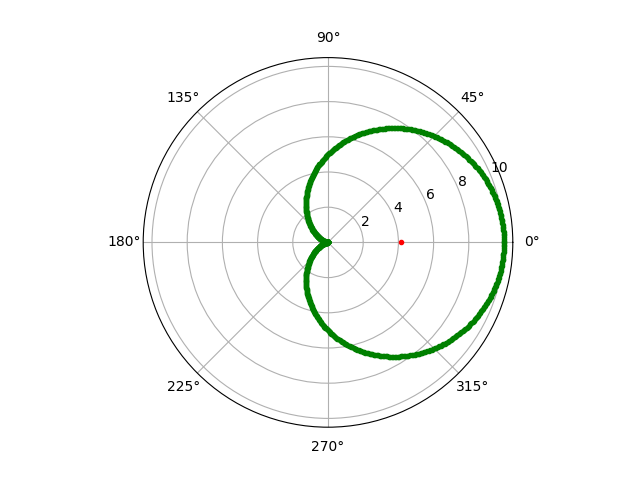
\includegraphics{Examples/output/center_of_gravity.png}
	\end{center}
	
	\newpage
	
	\subsection*{Exercise}
	\exercise{1}{
		Evaluate $\Iint{0}{x}{0}{1}{(x+y)\dyx}$
	} \vspace{1em}
	
	\exercise{2}{
		Find the $\Iiint{0}{x+\log(y)}{0}{x}{0}{\log(2)}{\hspace{-3em}\left(e^{x+y+z}\right)\dzyx}$
	} \vspace{1em}
	
	\exercise{3}{
		Find the area of positive quadrant of the circle $x^2+y^2=16$
	} \vspace{1em}
	
	\exercise{4}{
		Find the volume of tetrahedron $\displaystyle\frac{x}{2}+\frac{y}{3}+\frac{z}{4}=1$ bounded by the planes $x=0$, $y=0$ and $z=0$
	}
\end{document}